\documentclass[11pt,a4paper,titlepage]{article}
\PassOptionsToPackage{hyphens}{url}\usepackage{hyperref}
\usepackage[margin=1in]{geometry}
\usepackage[nottoc]{tocbibind}
\usepackage{graphicx}
\usepackage{amsmath}
\usepackage[ruled,vlined, linesnumbered]{algorithm2e}
\usepackage{makecell}
\usepackage{xcolor}
\usepackage[toc,page]{appendix}
\usepackage{subcaption}
\usepackage{tocloft}
\graphicspath{{./images/}}

\setcounter{tocdepth}{4}
\setcounter{secnumdepth}{4}
\setlength{\cftbeforesecskip}{6pt}

\author{Alex Campbell}
\date{}

\begin{document}

\begin{titlepage}
	\begin{center}
	\vspace*{1cm}
	
	\textbf{An Investigation into a Combined Approach to Solving the Travelling Salesman Problem}
	
	\vspace{1.5cm}

	Name: Alex Campbell
	
	Student ID: 1884111
	
	Programme Name: BSc Computer Science
	
	\vspace{1cm}	
	
	Supervisor: Dr Miqing Li
	
	\vspace{1cm}	
	
	Word Count: At most 9793 (according to Overleaf)
	
	\end{center}
\end{titlepage}
\setlength{\parindent}{0em}
\setlength{\parskip}{1em}


\section*{Abstract}

The travelling salesman problem is an incredibly popular and common problem, solving it is easy, yet solving it quickly is not. Many algorithms exist to find the exact answer, yet take a lot of time. If time is short, then maybe a method where we find a 'good enough' answer is suited instead. This thesis investigates a new kind of approximation algorithm, one where we combine a genetic algorithm with Christofides algorithm in order to see how it performs in comparison to its parts. The results were very interesting, showing this hybrid algorithm to perform best on all test data sets used. The results for the time taken however were underwhelming, and have significant potential to be improved and re-examined, due to inconsistencies and unexplainable occurrences within them. This thesis also experiments with editing Christofides algorithm to produce multiple outputs instead of just one, and seeing how these multiple outputs perform when all plugged into the genetic algorithm, with unsuccessful results using the shown approach.

\pagebreak

\tableofcontents
\pagebreak

\section{Introduction}

The Travelling Salesperson Problem (TSP) is an NP-Hard problem which is commonly found in combinatorial optimisation, theoretical computer science and operations research. It's a simple problem on the surface which simply states that "Given a list of cities and distances between each pair of them, what is the shortest possible route that visits each city exactly once and returns to the origin city?" \cite{TSPWiki}

This question appears deceptively simple, however with large sets of cities the search space becomes incredibly large, and as such computation time can be astronomical, since before you even start trying to compute the shortest tour, there are $n!$ different combinations to compute, assuming a complete graph. Clearly this meant another angle had to be taken for this problem.

As such many people decided to go for a more heuristic approach. So instead of trying to find the optimal solution with an infeasibly long time span, we would settle for a 'good enough' solution with a much lower time complexity, however since TSP is a combinatorial problem it is much more difficult to find the global optimum, with higher chances of falling into local optima.

And yet even with this said, there exists an algorithm that has been created more than 30 years ago (1976) that has been proven to be at most 50\% worse than the optimal solution for any given TSP problem and is known as Christofides algorithm. This algorithm has remained the best approximation available for over 30 years, and only recently (2020) has another, slightly more efficient algorithm been found \cite{TSP2020}, although though complete validity of it has yet to be verified.

However another way of finding approximate solutions is becoming more and more popular over time, and has its roots deeply set in evolution and natural selection, hence the name they are given: Evolutionary Algorithms. In essence these algorithms replicate the generational aspect of natural selection, taking the best individuals from a given population and 'breeding' them, these 'children' can then be tested to see if they perform any better than those in the population, and if so replace them, and this process continues to repeat until a certain criteria is met, which is usually a generation limit.

Genetic algorithms have already been used to try and solve the TSP which shall be discussed later, yet the major point of genetic algorithms is that you start with an entirely random population with which to create new solutions. If however we were to replace one of the population with a strong approximate solution ($x$), how would that affect the algorithm? Theoretically in the worst case scenario this genetic algorithm would simply return $x$, since if no better one can be found, then $x$ would remain in the population as the best solution, so we are no worse off compared to when we started the algorithm. However in the best case scenario the algorithm would produce a better approximate solution than $x$ and return this instead.

As such, in this thesis I will be investigating the usage of both the mathematical and algorithmic methods of finding a solution to the Travelling Salesman Problem, and thereby seeing if these methods can be combined into a singular algorithm and investigating it's effect.


\section{Background}

\subsection{Travelling Salesman Problem}
As explained briefly earlier, the TSP problem is a simple concept, a route that travels to every city in a given set exactly once and then returns to the starting position. TSP has been thoroughly worked on already, and as such plenty of data sets are available for TSP to be used on \cite{TSPRep1, TSPRep2}. Since the sites do contain the optimum solutions, or at very least the closest optimal solution, it makes evaluating our solution very easy since we can simply check the difference between our optimal solution for a given data set and their optimal.

\subsection{Genetic Algorithms}
Genetic algorithms take deep inspiration from natural selection and evolution in general. The very simplest description of a genetic algorithm is that given a starting population of predetermined size, calculate the fitness of each individual and choose the best of the population to 'reproduce' to create individuals that theoretically have the genes of both of these individuals, potentially giving it a higher fitness than its two parents. This child then has its fitness evaluated and if it is better than the worst individual in the population, it is added in place of it, this repeats for as many generations as we have chosen, and at the end of it we have a population of individuals who may have a better overall fitness than the initial population.

Most genetic algorithms take a very similar form, and though it is often altered for each individual case it is used in, most look very similar to the following pseudocode \cite{GAIntro}.

\begin{algorithm}[H]
\SetAlgoLined
\textbf{Initial Values:} generationNum = 0, generationMax = $N$\footnote{Where $N$ is a predetermined number of generations}\;
Randomly generate a population of size $P$ individuals to be used initially\;
Calculate the fitness of all $P$ individuals\;
Sort the population in descending order of fitness (assuming higher fitness is better)\;
\While{(generationNum $<$ generationMax)}{
	Pick the $M$\footnote{$ 2 \leq M \leq P$} best individuals from the start of the population\;
	\For{(each pair of parents in $M$\footnote{Selected randomly with replacement})}{
		Apply the crossover and mutation operators to produce two new offspring\;
		Evaluate their fitness\;
	}
	Replace the worst individuals in the population with the offspring assuming said offspring have a higher fitness than them \footnote{If all of the population are used to create new individuals then it will be the case that the entire population is replaced.}\;
	generationNum += 1\;
}
\caption{Pseudo code for a basic Genetic Algorithm}
\end{algorithm}

From the pseudo code it is very clear that genetic algorithms are very well suited for optimisation problems, either maximising or minimising the fitness of the individuals in the population. This means it is definitely a viable option to solve the TSP. However the pseudo code also shows there are a few operators and functions that need to be defined and explained before anything fruitful can be done.

\subsubsection{Individuals}

More of a clarification point more than anything, we need to decide what the individuals actually are within our problem of the TSP. Simply enough these individuals are solutions to the TSP, that is they are all routes that pass through each city and end back at the starting point, all without visiting a given city twice. The more important part however is how these routes should be stored in a way that the computer can work with.

Given that a solution to the TSP requires that all cities be used, a solution can simply be seen as an arrangement of these cities, whether this be as an array, list or simply a string. Any one of these formats would be suitable and effective to allow for the crossover and mutation functions to be applied, since regardless of format, all solutions will be of the same size.

\subsubsection{Objective Function and Fitness}

As stated briefly before, the TSP is an optimisation problem at its core, and genetic algorithms are powerful at solving such problems, and since this is a single objective optimisation problem in this case, the objective function itself is quite simple and can be formed from intuition:

$Minimise\; the\; following:$ \[F(\mathbf{x}) = \sum_{i,j \in \mathbf{x}} d_{i,j} \]

The objective function we want to minimise is $F(\mathbf{x})$ where $\mathbf{x} = \{x_1, x_2, ..., x_N\}$ is a given solution of the TSP problem, or in other words a permutation of all $N$ cities in our problem. $d_{i,j}$ represents the distance between cities $i$ and $j$ that are within $\mathbf{x}$, and we want to sum up the distances between them in order to get the cost of the full route.

So with that said it is blatant to see that the fitness function for any given route is simply the function we are trying to minimise, i.e.

\[\sum_{i,j \in \mathbf{x}} d_{i,j}\]

Which, stated simply, is the addition of all of the weights of the edges connecting our route, regardless of their value or type, i.e. distance, time etc.

\subsubsection{Mutation}

Mutation occurs after crossover,and there are many ways in which we can do mutations (but there are two that are used very commonly), one of which is to simply swap around two points in the tour (known as twors mutation \cite{GAMutations}), for example given:

\begin{center}\Large
Solution: 1\textcolor{red}{2}345\textcolor{red}{6}
\end{center}

Lets say we wish to swap towns 2 and 6, the solution would become:

\begin{center}\Large
Solution: 1\textcolor{red}{6}345\textcolor{red}{2}
\end{center}

This solution should be equally valid since the graph of the towns should be complete, that is every town is connected to every other town, so the route is still valid since an edge still exists.

Another method of mutation is to instead reverse a sub-tour within the tour itself (known as Reverse Sequence Mutation (RSM) \cite{GAMutations}), for example given the same example above, reversing the tour from 2 to 6 would give us:
 
\begin{center}\Large
Solution:1\textcolor{green}{23456}

Solution: 1\textcolor{green}{65432}
\end{center}

Naturally reversing a subtour is more computationally difficult than simply swapping 2 cities at random, however research has suggested that using RSM produces much stronger results compared to the other common methods, whilst simultaneously not being that much more difficult to understand \cite{GAMutations}. As such using RSM as the mutation operator for my own genetic algorithm would seem to be greatly beneficial.

It is important to note that mutation occurs by random chance, and so is not guaranteed to happen for any given child, otherwise the children might be too far spread across the search space and unable to close in properly to an optimum solution (either local or global).

\subsubsection{Crossover}

Crossover is another operator which heavily takes its inspiration from the process in meiosis with the same name. To explain it simply, crossover involves the swapping of genetic material, as an example we can see that 1\textcolor{red}{2}34\textcolor{red}{5}6 and 1\textcolor{blue}{2}34\textcolor{blue}{5}6 have the same numbers but differ in colour, if we swapped the number 5 between them (1\textcolor{red}{2}34\textcolor{blue}{5}6 and 1\textcolor{blue}{2}34\textcolor{red}{5}6), neither have changed in the sequence, yet their colours have changed, so neither sequence is missing anything, but they are now different. This is exactly what crossover is, it swaps genetic material such that no gene is missing, but they are now inherently different.

In normal genetic algorithms this process is identical to its biological counterpart, since the assumption is usually made that we are crossing over at identical points along both solutions, and as such no 'genes' are being lost or repeated. However in a solution for TSP, we cannot make this assumption, if we are to cross at a given point between two solutions, it may well be the case that two cities are repeated, and obviously this is not a possibility we can afford to have in a problem which strictly states every city must be visited exactly once. As an example of what I refer to take the following example and we wish to perform a crossover between the solutions between positions 4 and 5 like so:

\begin{center}\Large
Solution 1: 1534$|$26\\
Solution 2: 6543$|$21
\end{center}

If we now swap the solutions after this point accordingly we get:

\begin{center}\Large
Solution 1: \underline{1}534$|$2\underline{1}\\
Solution 2: \underline{6}543$|$2\underline{6}
\end{center}

Underlined you can see we now have repeated cities, there is also the issue where solution one now doesn't include 6 and solution 2 doesn't include 1, so neither can be tours for the TSP.

As such we must look at a different method of crossover, which takes the same core concept, yet avoids this issue detailed above. As a matter of fact there are a fair amount of different crossover operators that have been designed exactly for this purpose and shall be detailed shortly.

\section{Literature Review}

\subsection{Different Crossover Operators}

\subsubsection{Partially Mapped Crossover}

In this crossover operator \cite{GACrossover}, proposed by Goldberg and Lingle, two random cut points are used as its basis, instead of doing a singular crossover point like demonstrated above. After the cuts have been made one of the parents has its subroute mapped onto the other parent's subroute before the other remaining information is exchanged between the two parents. As an example take the following two parents who have the crossover points marked in the same way as before \cite{GACrossover}:

\begin{center}\Large
Solution 1: (348$|$271$|$65)\\
Solution 2: (425$|$168$|$37)
\end{center}

In this scenario the mapping is between 2, 7, 1 and 6, 1, 8. So we swap these around and make two new children based off of them:

\begin{center}\Large
Child 1: (XXX$|$168$|$XX)\\
Child 2: (XXX$|$271$|$XX)
\end{center}

The next stage is to fill in the Xs with the appropriate cities from their corresponding parent, checking of course first that a city is not being repeated. (So Child 1 will receive Parent 1's cities and vice versa):

\begin{center}\Large
Child 1: (34X$|$168$|$X5)\\
Child 2: (4X5$|$271$|$3X)
\end{center}

From here we need to fill in the remaining Xs that have conflicts with other cities, the first X in child one would have originally been 8 from parent 1, though since there is already an 8 in child 1, we check the order which shows 8 is in the same position as 1, so we then check if 1 is in the child, which turns out to be true, so once again we check and see 1 lines up with 2, we check if 2 is in the child and it is not, hence the first X becomes a 2. We do the same for the second X in child 1, which should have been a 6 yet it cannot be, the mapping shows 6 is lines up to 7 so we test 7 and it does not conflict, therefore we have Child 1 being equal to:

\begin{center}\Large
Child 1: (342$|$168$|$75)
\end{center}

We compute child 2 in exactly the same way which then gives us:

\begin{center}\Large
Child 2: (485$|$271$|$36)
\end{center}

And therefore we get two output children to test the fitness with and add to the population if necessary.

\subsubsection{Order Crossover}

Another crossover operator is the order crossover proposed by Davis \cite{GACrossover}, and it builds offspring by choosing a sub tour from the parents and preserving the relative order of cities in the other parent. As an example:

\begin{center}\Large
Solution 1: (147$|$258$|$36)\\
Solution 2: (482$|$653$|$71)
\end{center}

The offspring are created first by the sub tour of their respective parents:

\begin{center}\Large
Child 1: (XXX$|$258$|$XX)\\
Child 2: (XXX$|$653$|$XX)
\end{center}

Then from the opposite parent of each solution, we take the list of cities starting from the second cut point, and removing any already present in the 1st child, e.g. in this case we take the tour 7,1,4,8,2,6,5,3 then remove 2,5 and 8 to give 7,1,4,6,3 which is then placed in the 1st child starting from the 2nd cut point to give:

\begin{center}\Large
Child 1: (463$|$271$|$71)
\end{center}

And child 2 is made in the same way:

\begin{center}\Large
Child 2: (728$|$653$|$14)
\end{center}

\subsubsection{Cycle Crossover}

Cycle crossover is an operator which takes a different approach compared to the other two detailed above. It works by splitting the parents into 'cycles' and then alternating adding each one to their children. It is an algorithm which is best described through an example, however we must use a different example from the one used previously for reasons that shall be discussed afterwards \cite{GACrossover}:

\begin{center}\Large
Solution 1: (12345678)\\
Solution 2: (85213647)
\end{center}

We start by picking one of the starting cities, in this case 1 or 8. In this case we will pick 1, and this is added to the first child:

\begin{center}\Large
Child 1: (1XXXXXXX)\\
\end{center}

We then look at the city in the corresponding position of parent 2 and go to that appropriate position in parent 1, so that we can add it to child 2, in this case the parent 2 city is 8, so we go to position 8 whilst also adding it to child 1:

\begin{center}\Large
Child 1: (1XXXXXX8)\\
\end{center}

We continue this, next getting a 7:

\begin{center}\Large
Child 1: (1XXXXX78)\\
\end{center}

And then a 4:

\begin{center}\Large
Child 1: (1XX4XX78)\\
\end{center}

From here the corresponding point is 1, however since we already have used 1 a the very beginning, it is already in the list and so that is the end of this 'cycle'. At this point we fill in the remaining missing cities with the ones from the second parent to give:

 \begin{center}\Large
Child 1: (15243678)\\
\end{center}

We can then do the same for child 2 which would give us:

\begin{center}\Large
Child 2: (82315647)\\
\end{center}

As I mentioned earlier we had to use a separate example from the one we used for the other crossover operators in this case, this was because of the drawback of this technique. If you used this operator on our other examples, you would find that both children would end up exactly the same as their parents, which is clearly a very large waste of computation.

In a paper by Abid Hussain et al. \cite{GACrossoverPerformance}, they investigate the performance of each of these operators along with many others to see which would lead to the best solutions in a given number of iterations, the results of this experiment showed that partially mapped crossover and cycle crossover both performed very similarly, but were a significant margin away from the performance of the order crossover on the BERLIN52 instance which this experiment was run on. As such, due to the relative simplicity of order crossover compared to the other two examples, and cycle crossovers drawback of potentially producing identical children, it strongly suggests that the most suitable crossover operator to use in our genetic algorithm would be the order crossover.

\subsection{Different Algorithms for TSP}

\subsubsection{Brute Force Algorithm}

Much like the name suggests, a brute force algorithm doesn't really solve the problem in a clever way, it just brute forces a solution by testing every single solution within the search space of the optimisation problem. When the problem we are dealing with is small, this algorithm works exceedingly well, and since it is just iterating through every possible solution, it is very easy to implement, and for smaller problems it isnt really worth creating a more complex solution when a brute force approach will find an optimal solution perfectly well \cite{DiffAlgs}. As we said the algorithms main downside is its time complexity, as the size of the problem increases, this algorithm becomes inefficient incredibly fast.

This algorithm isn't really suited for this project however, since the problems I wish to attempt within this will be very large by nature, and a brute force approach is definitely not well designed for that.

\subsubsection{Greedy Algorithm}

Greedy algorithms are a step above brute force algorithms, they have a much smaller time complexity ($O(n)$) and are equally as easy to implement. They are still better suited for smaller search spaces however but not for the same reasons as the brute force algorithm. Greedy algorithms take a very short sighted approach to finding a solution, at each stage it takes the shortest route it can to another city (assuming it hasn't been visited already) until all of the cities have been visited and it returns to the starting point. The main downside of the algorithm is its tendency to get stuck in local optima, which is best described with a diagram.

\begin{figure}[ht]
	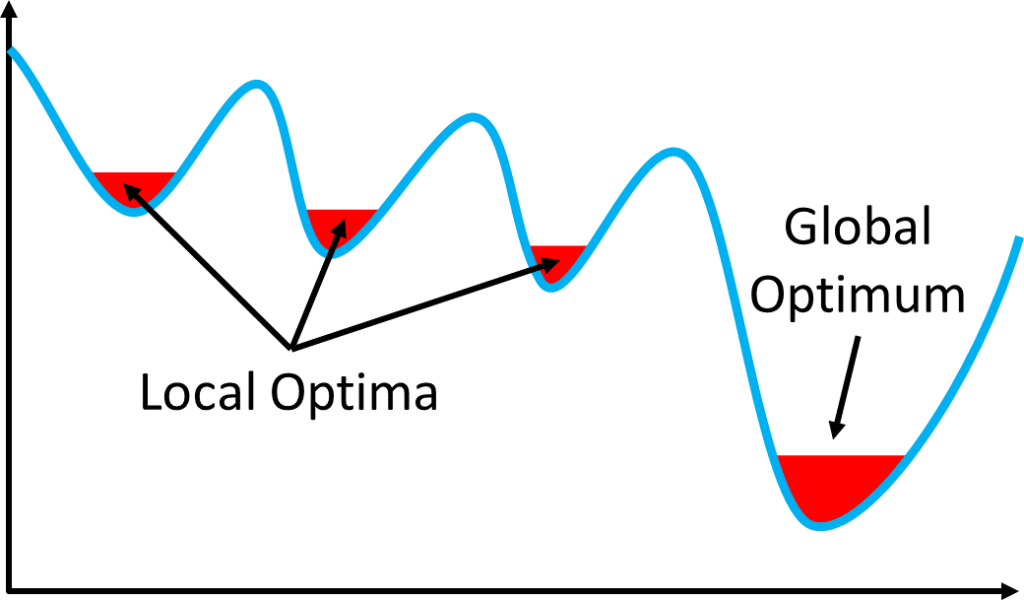
\includegraphics[scale=0.3]{LocalGlobalOptima}
	\centering
	\caption{Full Graph}
\end{figure}

When the greedy algorithm travels down the line,it will continue to do so until it reaches an optima, be that local or global, it does not travel across the whole search space so it easily gets stuck in one of these 'dips' and will not reach the global optimum. In other words by taking the shortest route every time, we may miss a better route which is shorter overall but takes a longer path between some cities. This is much more of an issue for larger search spaces than smaller ones, but since we will be using larger search spaces, it makes this algorithm unsuitable for this experiment.

\subsubsection{Held-Karp Algorithm}
The Held-Karp algorithm is currently the best available for finding the optimum solution with a time complexity of $O(n^2 2^n)$, which whilst not great from a practical stand point, is leagues ahead of its brute force counterpart. This being said with its complexity still being quite high, it is unsuitable for very large data sets as it suffers greatly at these levels \cite{HeldKarpAlg}.

As a brief mention of the algorithm, it calculates suboptimal shortest paths that satisfy the following, and gradually builds them up until it reaches its answer:

\begin{enumerate}
\item Each route must traverse an explicit set of nodes.
\item Each route must end on a specific node.
\end{enumerate}

As stated before even though this is the best for finding the optimal solution to TSP, its time complexity is still exceptionally large. Furthermore for the purposes of this project it is unsuitable since it is already guaranteed to find the optimum,and combining it with any other method will be of no use, only serving to push the time required even further. 

\subsubsection{Christofides Algorithm}
Even with the algorithm having been created over 30 years ago in 1976, there has yet to be another verified algorithm at this time that can produce more optimal approximate solutions to the TSP problem than this. This algorithm has been proven to be at most 50\% worse than the optimal solution whilst having an $O(n^3)$ time complexity where n is the number of cities for which we are trying to solve the problem. \cite{ChrAlg} If we instead look at the best algorithm currently available to solve the TSP (aka the Held-Karp Algorithm) we can see that its complexity is $O(n^2 2^n)$ \cite{HeldKarpAlg} which, whilst astronomically better than the original $O(n!)$, is significantly worse than the approximate solution that Christofides algorithm provides.

This is often the case with such computationally expensive problems, a balance must often be made between finding the optimal solution, and finding a solution in an appropriate amount of time. The Held-Karp algorithm focuses more on finding the optimum answer rather than finding it in a feasible amount of time, whereas Christofides Algorithm was designed to find as best an approximation as it can whilst still having a relatively feasible computation time which is what can make it so appealing to use. 

One of the strong points about Christofides algorithm is just how simple it is, having only 4 or 5 major steps (many sources combine steps 4 and 5 whilst others do not \cite{ChrAlgSlides, ChrAlgSteps}) even if these steps are more likes processes themselves. 

Nonetheless the steps to this algorithm are as follows:
\begin{enumerate}
	\item Find a minimum spanning tree $T$.
	\item Find a minimum weight perfect matching $M$ for the odd degree vertices in $T$.
	\item Calculate $M \bigcup T$.
	\item Find an Euler tour of $M \bigcup T$.
	\item Remove any repeated vertices.
\end{enumerate}

\begin{figure}[ht]
	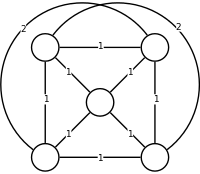
\includegraphics[scale=0.75]{WikiCompleteGraph}
	\centering
	\caption{Full Graph}
\end{figure}

\clearpage
As stated the process is compressed into few steps and is quite simple to understand, and yet creating this algorithm within a programming language is more complex than one would initially assume. Finding a minimum spanning tree (Figure 3) of the full graph (Figure 2) is quite simple, the two most common algorithms known for solving this are Prims and Kruskals, both of which are effective methods with time complexities of $O(n)$ and $O(n^2)$ respectively \cite{PvKTime} though choosing one or the other is mostly affected by the number of edges within the graph we are finding the minimum spanning tree for, with Prims being more suitable if there are a large number of edges, and Kruskals if not.

\begin{figure}[ht]
	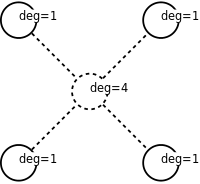
\includegraphics[scale=0.6]{WikiMinSpanTree}
	\centering
	\caption{Minimum Spanning Tree}
\end{figure}

The minimum weight perfect matching of $T$ (Figure 4) is accomplished by finding $\frac{T}{2}$ edges which 'link' together every vertex in $T$ by the shortest edge possible. For this one of the most common algorithm in use appears to be the blossom algorithm and has a time complexity of $O(n^2 m)$ in the worst case where $n$ is the number of vertices and $m$ is the number of edges \cite{BlosAlg}.

\begin{figure}[ht]
	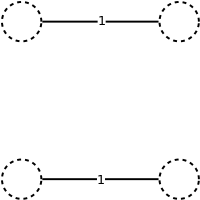
\includegraphics[scale=0.6]{WikiMinMatch}
	\centering
	\caption{Minimum Weight Perfect Matching}
\end{figure}

From here we simply calculate the union of $M$ and $T$ (Figure 5), including any of the repeated edges that may be present, before moving onto the Euler tour. A Euler tour is simply a tour of the graph which visits each edge exactly once, regardless of starting or ending vertex (Figure 6).

\begin{figure}[ht]
	\centering
		\begin{minipage}{0.45\textwidth}
			\centering
			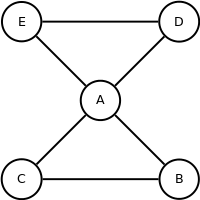
\includegraphics[scale=0.5]{WikiComb}
			\caption{$M \bigcup T$}
		\end{minipage}\hfill
		\begin{minipage}{0.45\textwidth}
			\centering
			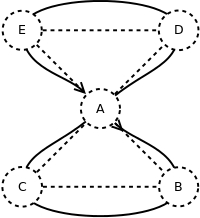
\includegraphics[scale=0.5]{WikiEulerTour}
			\caption{Euler Tour}
		\end{minipage}\hfill
\end{figure}

Then need to remove any repeated vertices within our tour and replace them with the direct edge between those vertices, and once this is done we have the algorithms output (Figure 6).

\begin{figure}[ht]
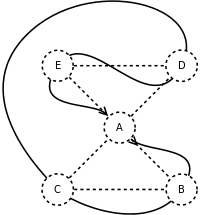
\includegraphics[scale=0.6]{WikiRemove}
\centering
\caption{Christofides Algorithm Output}
\end{figure}

(Figures 1-6 taken from: Wikipedia: Travelling Saleman Problem \cite{TSPWiki})

With this algorithm output we now have a solution to the TSP for our specific graph, and this solution is guaranteed to be within 50\% of the optimum \cite{ChrAlg}, which is significantly better than trying to calculate the true optimum for a very large graph in an infeasible amount of time. However there is clear room for improvement, since for these very large graphs, a solution that is 50\% worse is still drastically longer than the optimum. Making improvements on this is therefore exactly what I plan to do, as it gives us a good basis to work other algorithms off of, as is the point of this project.

\section{Implementation}

\subsection{Data Sets}

For an investigative project such as this, it makes sense to use a variety of different data sets which will appropriately represent the different possible situations this algorithm could be used in, as such I have used three data sets of varying sizes to analyse my algorithm with. These data sets have all been taken from the same source \cite{TSPRep1} which also contain the optimum lengths of the tours for each data set available on the site. It is worth noting that there are no units for said distances, yet this point is negligible for the purposes of this project. I have chosen three data sets of varying sizes to see how the algorithm will fare in each of them, these data sets are the cities of Qatar, Zimbabwe and Oman which have 194, 929 and 1979 cities respectively. Each of these data sets are encoded as qa194 (Qatar), zi929 (Zimbabwe) and mu1979 (Oman) and shall be referred to as such from now on for simplicities sake.
\pagebreak

The optimum lengths for the datasets are as follows:

\begin{center}
\begin{tabular}{c | c}
Data set & Optimum Length \\ [0.5ex]
\hline
	qa194 & 9352 \\
	zi929 & 95345 \\
	mu1979 & 86891
\end{tabular}
\end{center}

Each of these data sets is stored in a file format known as tsplib which gives some basic details on the data set along with the points of said data set.The details of the data structure are not really relevant, but the important aspects are simply that each city is stored with a number identifying it (quite simply a list from 1 to n) and next to said number is its coordinates, and from this it is simple to calculate the distances between the cities by just using the required distance metric (which is also specified within the file, and in the case of these data sets, it is all euclidean distance).

\subsection{Data Structures}

The travelling salesman problem involves dealing with multiple graphs of cities and the roads connecting them, as well as keeping track of multiple individuals which each represent a given tour around said graph. As such it made perfect sense to use some specific data structures for these to allow the usage of them to be as intuitive as possible. The graph itself was stored as a list of nodes, a 2D array of the edges and a string representing its name. This is nothing particularly outlandish but allows for the graph to be accessed easily enough. The edges were best stored as a 2D array since each pair of cities had an edge between them, as such the entirety of the array would be filled (bar the diagonals, which would represent the edge of a given city to itself). It would be possible to calculate the distance between each city as needed instead of storing them all at the beginning, however this would be less efficient in my opinion due to the number of times a given edge would have to be calculated, whereas storing them outright would sacrifice some space in order to reduce execution time. The nodes were simply small data structures which contained the x and y coordinates of each city along with its identifier (number in this case).

The other major data structure would be the "Individual" class, which is what a given solution to the TSP would be stored as. The individual contains a list of the nodes in the order of which they would be visited, along with the 'fitness' of the individual (aka the length of the tour) which is calculated upon an instance of an individual being created. The data structure does not store the edges of the individual as these can be found out very quickly from the tour itself, simply searching the 2D array with the indexes being two consecutive nodes in the tour, this was to prevent any more space being used than necessary.

\pagebreak

\subsection{Parameters}

Genetic algorithms come with a fair few parameters to tweak, all of which can make quite the significant difference upon the results obtained and as such need to be optimised. The important ones are as follows:

\begin{itemize}
\item Population Size: Number of individuals within the population.
\item Number of generations: Maximum number of generations to be computed.
\item Number of calculations: Population * Generations, used to keep the general number of calculations about the same when tweaking with generations and population size.
\item Crossover Chance: Chance of crossover happening.
\item Mutation Chance: Chance of mutation happening.
\end{itemize}

\subsubsection{Generations and Population}

\begin{table}[h]
\centering
\begin{tabular}{c | c | c | c}
\makecell{Data set} & \makecell{Population: 200 \\ Generations: 25000} & \makecell{Population: 1000 \\ Generations: 5000} & \makecell{Population: 2000 \\ Generations: 2500} \\ [0.5ex]
\Xhline{1.5pt}
	qa194 & 10540.6556793449 & 10543.3664673219 & 10109.16049177478 \\
\hline
	zi929 & 138258.542848618 & 124442.958821215 & 222572.64170034693 \\
\hline
	mu1979 & 634606.350605636 & 351729.696875395 & 2703446.74385851

\end{tabular}
\caption{The results in the table are for the pure genetic algorithm, not the hybrid algorithm}
\end{table}

Before discussing the results above, it is important to note that usually for genetic algorithms, smaller population sizes with larger generation numbers do better than larger population sizes. With that being said we can see here that the datasets actually react in the opposite way, the qa194 data set gives incredibly similar results for all, so they can be disregarded in this instance, however for the zi929 and mu1979 datasets we can see that the smaller population does worse on both accounts, and extremely so in the case of the mu1979 data set where is it around 300,000 worse. For a population size of 2000 it was once again very similar for the qa194 data set, but interestingly for the zi929 data set it was significantly worse than both whilst the mu1979 was a significant amount better instead. However since a larger population leads to a larger number of parents, it means the execution time of the program is significantly greater, and as such for this reason I have decided to stick with the 1000 population size as to balance out the results for all 3 datasets as well as decrease the running time of the program, yet if better results are required and time is of no concern, using this larger population size could be beneficial.

\subsubsection{Mutation and Crossover}

The other important parameters are the mutation and crossover chance, the mutation operator is applied after the crossover and applies to the children when they are generated, the crossover chance is basically the chance of two of the parents 'mating' to create two new children, if the crossover chance is not met then the two parents are simply carried forward as the children, essentially copying them.

\pagebreak

In regards to optimising them I used the same method as used for the population and generation sizes, as shown in the table below:

\begin{table}[h]
\centering
\begin{tabular}{c | c | c | c}
Data set & Mutation: 0.1 & Mutation: 0.4 & Mutation: 0.9 \\ [0.5ex]
\Xhline{1.5pt}
	qa194 & 10220.556448011208 & 10042.534388187263 & 10307.448956457112 \\
\hline
	zi929 & 180637.17314356696 & 154080.72513430865 & 289831.6821760032 \\
\hline
	mu1979 & 1273721.9043312161 & 1461183.9174761462 & 2738641.7549757827

\end{tabular}
\caption{Once again the results in the table are for the pure genetic algorithm, not the hybrid algorithm}
\end{table}

Here we can see that a mutation of 0.9 is significantly worse on the larger datasets than the other two mutation values, and this is to be expected since mutation rates are never supposed to be as high as this, we can also see that the differences between 0.1 and 0.4 aren't as large as expected, however between the two a mutation of 0.4 does better generally. The largest data set does not have a relatively large difference between the two, and this can be accounted for with the general randomness of the genetic algorithm, if the difference was closer to $500,000$ or more I would count this as a more significant value. As such I shall choose a mutation of 0.4 for the results of the hybrid.

And then below we see the same for optimisation of the crossover chances. In general the chance for crossover should be quite high whilst the mutation percentages tend to be a lot lower and we can see that these chances definitely reflect this general trend.

\begin{table}[h]
\centering
\begin{tabular}{c | c | c | c}
Data set & Crossover: 0.1 & Crossover: 0.4 & Crossover: 0.9 \\ [0.5ex]
\Xhline{1.5pt}
	qa194 & 10536.952603005655 & 10152.56527247845 & 10412.855764138969 \\
\hline
	zi929 & 193926.6438033023 & 161403.49362711725 & 153977.29243174416 \\
\hline
	mu1979 & 2539262.528786441 & 1874666.6607498457 & 1451559.7225074822

\end{tabular}
\caption{Results in the table are for the pure genetic algorithm, not the hybrid algorithm}
\end{table}

For the above data we can see that a crossover of 0.1 does significantly worse on the largest data set and does moderately worse for the medium sized one, the smallest data set once again doesn't really tell us much in all three cases since the variation is always incredibly minor, yet the other two show that a crossover of 0.9 has the best results in both cases compared to a crossover of 0.4, this matches what is expected since in general a higher chance of crossover is usually better. As such can see the best values for mutation and crossover are 0.4 and 0.9 respectively and therefore these are the values I used for my hybrid algorithm.

\subsection{Christofides Algorithm}
The implementation of Christofides algorithm was mostly unimpeded, so only the important aspects shall be mentioned.

\subsubsection{Find a minimum weight perfect matching}
This would have been a difficult algorithm to implement, and even more so to do in an efficient manner, as such for this stage and one other I used a library that is freely available \cite{KolMinMatch} which contains a function to calculate this exactly, the only awkward part of this was manipulating my graph data structure into a form that the algorithm would accept and be able to use properly, however this was more time consuming than actually difficult to accomplish.

\subsubsection{Find a euler tour of the union graph}
In the same manner as the minimum weight perfect matching, calculating a euler tour for the union graph would have been difficult to implement quickly and efficiently, and implementing this isnt the main part of this project, and as such another library was used \cite{HeirEulTour} to calculate the tour. The calculated tour then needed to be converted back into my own data structure which was not a complicated process at all, it simply required converting the edges into a list of cities instead.

\subsubsection{Remove repeated vertices}
This step is incredibly easy to do if you decide to do it simply, just go through the list checking each city and seeing if it appears again further down the line, then you just remove any that were found afterwards and you have your completed tour of the cities, however part of my project was to test to see if multiple individuals being added to the population would lead to a better or worse result, and it is this stage here in which the crux of that investigation begins and how this function can become quite a bit more complex, and that shall be discussed in more detail later.

Overall these steps together will create a singular tour which will be at most 1.5 times worse than the optimum tour around a given graph. This individual can then be plugged directly into the population of the genetic algorithm and we can then allow to generations to run as many times as we deem necessary to achieve fruitful results.

\subsection{Multiple Christofides Individuals}
As stated just a little bit ago we can change the simple step of removing repeated vertices to be quite a bit more complex in order to generate multiple individuals from it. Notably each of these multiple individuals will be worse than that of the singular individual, however the entire purpose of a genetic algorithm is to work with worse individuals and create better ones from them, so perhaps having multiple worse individuals that are spread more over the search space will allow the algorithm to find its way to the global optima (or somewhere close) much more quickly.

With this in mind the following code is what was produced to create said individuals, the specifics are not incredibly important and only the more important aspects shall be explained below.

\begin{figure}[ht]
	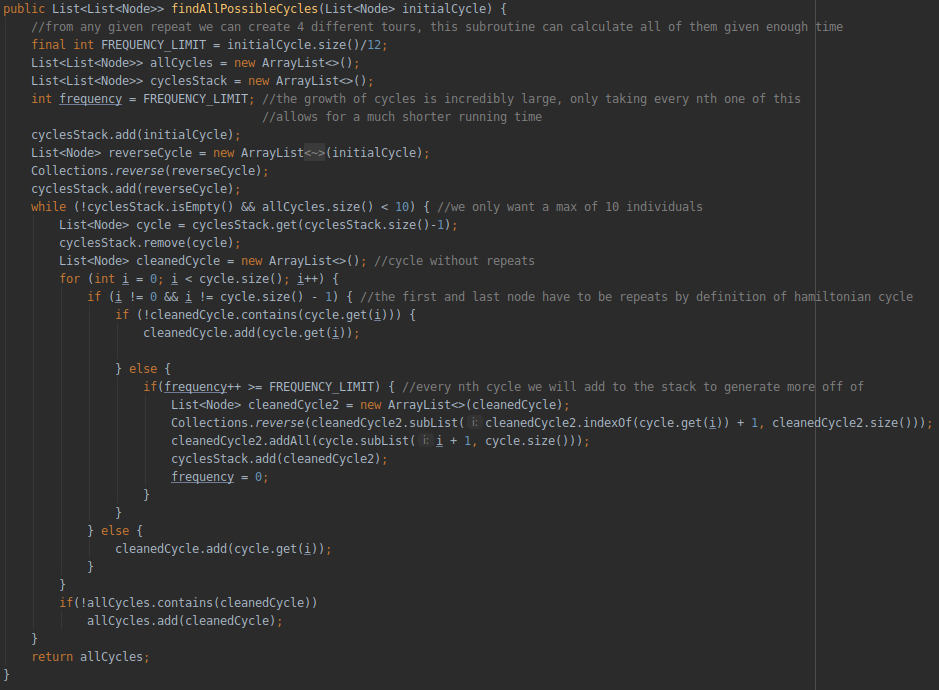
\includegraphics[scale=0.45]{MultiChrisAlg}
	\centering
	\caption{Code for multiple Christofides individuals.}
\end{figure}

The first important thing to note is how this algorithm works overall, for any given repeat we encounter we can remove either the first instance or the second, doing this will lead to two separate tours which we can then iterate on again to remove the other repeats. Furthermore, not only can we remove either one, we can also reverse the tour and remove each of them. As such for every repeat we can create 4 different tours, and therefore it is obvious to see that the number of tours we can create will grow exponentially fast, because of this the time taken by the algorithm would be far too long in most tour sizes to be of any use.

With this in mind my code works by adding each of these newly created tours onto a stack of tours which will be iterated on. We still have to tackle the issue of the exponential growth, and to do this I used a "FREQUENCY\_LIMIT" which decided how many tours would be added to the queue and how many would simply be discarded. e.g. if the frequency limit was 5 then only every 5th tour generated would be added back onto the stack, and as such a lot of the tours could be discarded, and we do not need many of them in the first place, since the idea of this is to add a few individuals to the population, instead of entirely overriding it, and with this in mind there is a condition to stop the execution once 10 tours have been reached.

When every nth tour is reached, the function will create a copy of the tour and reverse it, then add it to the stack to be worked on each, and the program then continues on its current tour to remove all of its repeats before in order to add to the final list of tours which we can then use. The frequency chosen here was the size of the tour divided by 12, this was to try and make said size dynamic, such that smaller tours would have the chosen tours closer together and the larger tours further away, and this in turn was to create as large a variety of tours as possible, instead of ending up with many tours that were incredibly similar, as this would simply lead to getting caught in a local optimum very quickly.

Once execution of this is finished all 10 of the tours are to be added to the generation, with the other 990 (to give 1000 individuals) being randomly generated which will then be used by the genetic algorithm for 5000 generations on each data set.

\section{Results}

With everything now in place we can look into the results achieved by the algorithms and explain how and why they are the way they are.

\subsection{Algorithm Evolution}

The first results I will show are the evolutionary graphs of the singular hybrid algorithm alongside the pure genetic algorithm, so that we can see how their individuals are improving as the generations go by. The full tables of data for each of the graphs can be found in appendix A.

It is important that the layout of the graphs is first explained. There are two lines on each graph, the blue line represents the results of \textbf{just} the genetic algorithm and the orange line represents the results of the hybrid algorithm, and the x-axis represents the generation number. Most importantly is the scales, the results for genetic algorithm and hybrid algorithm were vastly different, so two different scales have had to be used in order to show both lines on one graph, and this was the best way to represent the data as it most clearly shows how the trends of both differ. The scale on the \textbf{left} of each graph represents the genetic algorithm (blue line) and the scale on the \textbf{right} represents the hybrid algorithm (orange line).

\subsubsection{Qa194 Data Set}

\begin{figure}[ht]
	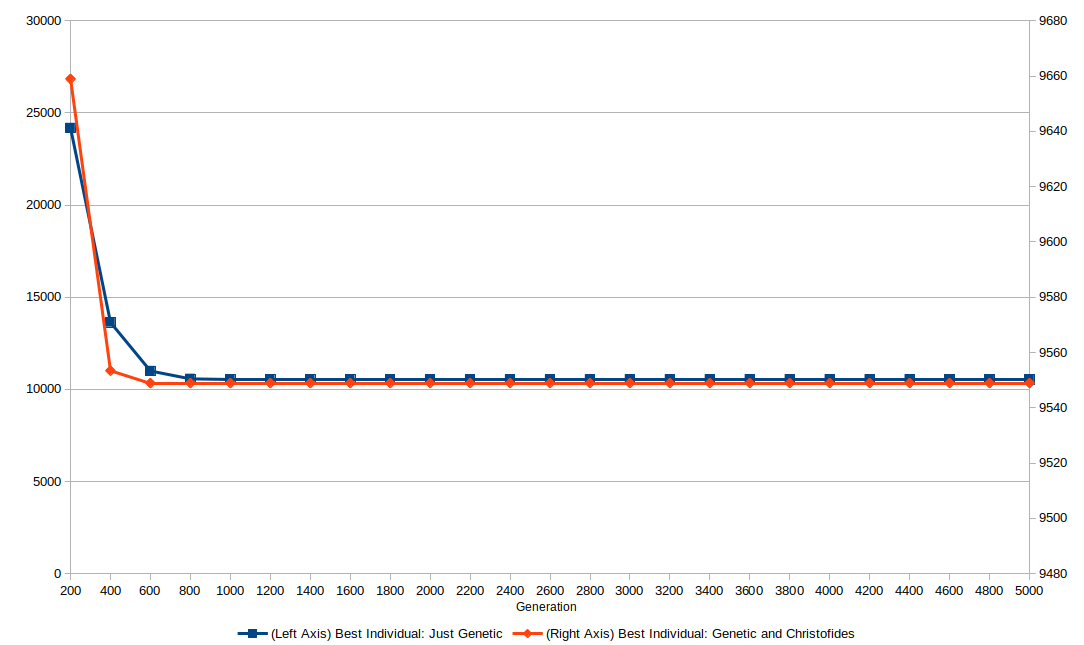
\includegraphics[width=\textwidth]{qa194Evolution}
	\centering
	\caption{qa194 data set evolution}
\end{figure}


The first thing that immediately jumps out on this graph is how quickly both of these algorithms plateau, and deceptively it appears like both have plateaued very close to one another, however one look at the scale shows that there is a significant difference between the two values they have stuck with. The values specifically are $10543.3664673219$ for the genetic algorithm and $9548.91872392524$ for the hybrid. As we can see the hybrid algorithm hits the plateau about the same time as the genetic algorithm, however said plateau is hit at a tour which is 1000 better than the genetic algorithm, which means that even if they have stopped improving at the same time, the local optima that they have both become trapped in are certainly different (and in the hybrids case, better).

As such we can see in this small data sets case, after the same number of generations (approximately 800) we have a much better result with the hybrid compared to the genetic algorithm, and on top of this still we can see that the hybrid algorithm has been able to reach around 200 from the global optimum ($9352$) compared to the genetic algorithm which is around $1200$ off, which is a significantly better result.

\subsubsection{Zi929 Data Set}

\begin{figure}[ht]
	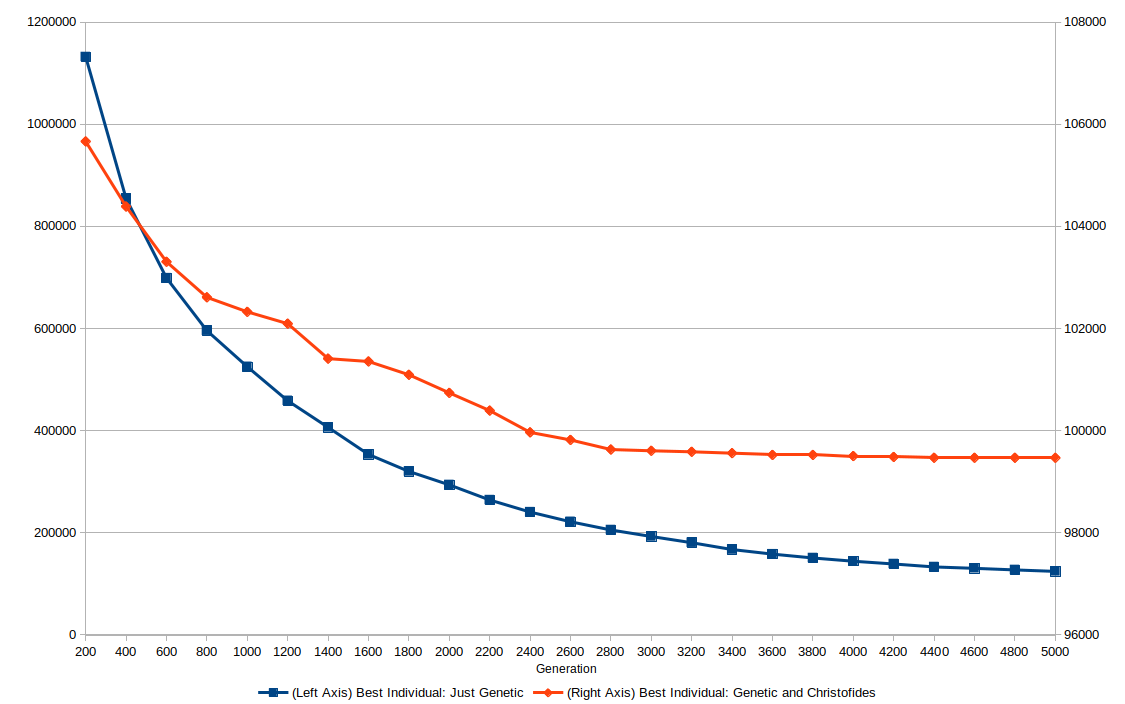
\includegraphics[width=\textwidth]{zi929Evolution}
	\centering
	\caption{zi929 data set evolution}
\end{figure}

This evolutionary graph shows much more interesting data compared to the previous one, as we can see  both algorithms take a larger number of generations before they start to plateau, and the genetic algorithm only just starts to plateau at the 5000th generation, whereas the hybrid seems to have plateaued closer to the 3000th generation.

If we look at the general trend of them, we can see that the genetic algorithm starts decreasing very quickly and then trails off, decreasing less and less until it stops, and this is the expected trend, however the hybrid algorithm has a stranger shape to it, despite the hybrid algorithm using solely the genetic part at this point, the rate at which the individuals improve is not as consistent as the pure genetic algorithm, instead decreasing at strange intervals, before eventually trailing off at around the 3000th generation. That being said, the results of the genetic algorithm are still significantly worse than that of the hybrid algorithm. The genetic algorithm had a final result of $124442.958821215$ whereas the hybrid algorithm had a result of $99467.6109972511$  which is around $30,000$ better. In comparison to the global optimum ($95345$) we can see that once again the hybrid algorithm gets very close respective to the size of the tours, getting within $4000$ whereas the genetic algorithm was around $29,000$ off, which is obviously significantly worse.

With this being said it appears neither of these had quite reached a true plateau, as the table within appendix A2 shows that they were both still improving, if only marginally, as such given more time it would be interesting to see at what point they would both plateau fully.

\subsubsection{Mu1979 Data Set}

\begin{figure}[ht]
	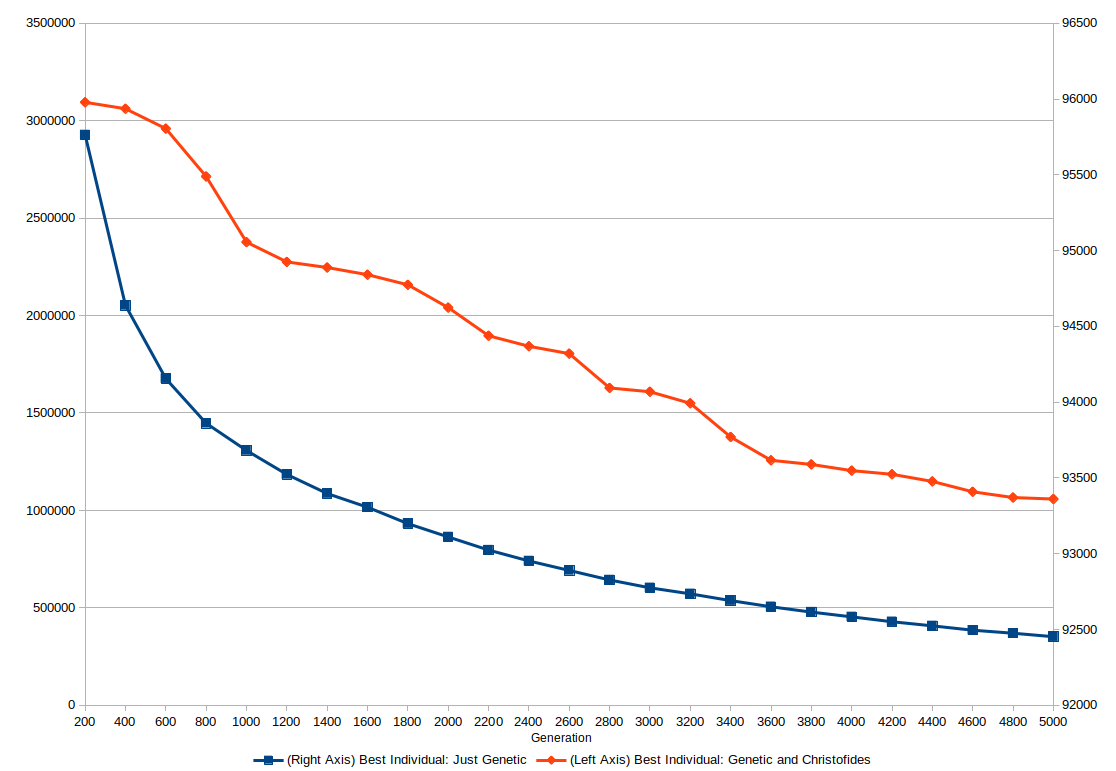
\includegraphics[width=\textwidth]{mu1979Evolution}
	\centering
	\caption{Mu1979 data set evolution}
\end{figure}

Finally we have the largest data set, and we can notice that the trends for each algorithm are fairly similar to what they were on the previous data set, the genetic algorithm starts decreasing a lot quicker before slowing down, whilst the hybrid algorithm is significantly more unpredictable to find a consistent trend with. What else we can see is that neither have plateaued yet, and as such this data could definitely do with being ran again with a higher generation limit if more time was available, as the genetic algorithm and the hybrid algorithm both have capacity for further improvement.

Nevertheless analysing what data is here we can see that the scales this time are ludicrously different, the starting point for the genetic algorithm is around $3,000,000$ whereas for the hybrid it is around $96,000$ and as such the hybrid algorithm is already at a significant advantage before any generations have been executed. Despite this we can see that the genetic algorithm does improve a lot, down below $500,000$ and the hybrid algorithm also improves, though not at all to the same degree.

However if we look at the final results in this case we can see there is no contest between the two; the genetic algorithm had a result of $351,729.696875395$ and the hybrid algorithm had a result of $93,360.7690694728$. With the optimum being $86,891$ we can clearly see that the hybrid algorithm is insurmountably better, with it being only $7,000$ worse compared to the genetic algorithm being more than 4 times worse than optimum.

\subsection{Mean Results}

Christofides algorithm has a degree of randomness within it, and genetic algorithms are built upon randomness as a premise, as such it would certainly not be a stretch to say the above results were a one off, and that is true to some degree, as the chances of finding these exact results once again when running the program are slim to none. Nevertheless we can analyse how the program handles in the mean case, and see how the results may deviate from one execution to another. With this in mind we have the following results that have been collected to investigate this very issue:

\begin{figure}[ht]
	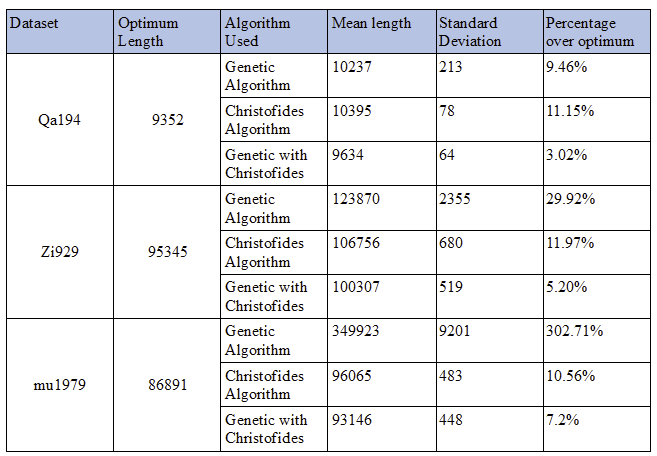
\includegraphics[width=\textwidth]{MeanResults}
	\centering
	\caption{Mean, standard deviation and percentage over optimum of the algorithms over 30 executions}
\end{figure}

Starting with the qa194 data set we can see that the genetic algorithm on its own fares quite well in getting an approximate result, getting a mean of 9.46\% over the optimum whereas Christofides algorithm actually fares slightly worse with 11.15\% over the optimum. This being said Christofides algorithm is much more consistent with the results compared to the genetic algorithm which can vary around 3x more. Either way the clear winner is the hybrid algorithm which manages to be within 3.02\% of the optimum along with also having the smallest deviation out of the 3 algorithms, therefore meaning it is not only the best in this instance at getting an approximate answer, but also the most consistent, which is an extremely good result over the 30 executions. Therefore for this smaller data set it is clear the hybrid algorithm is significantly better, and the reasoning for this is most likely related to the local/global optimum dilemma mentioned before. The genetic algorithm has to work from pure randomness to try and get close to the global optimum, and so is definitely vulnerable to getting stuck in local optima along the way, whereas the hybrid algorithm is already placed much closer to the global optimum and as such is less likely to get stuck in a local optimum that is as far away as the genetic algorithm.

The second data set (zi929) shows similar results; the genetic algorithm has a mean tour length that is 29.92\% worse than the optimum which is considerably worse than Christofides algorithm which reaches 11.97\% from the optimum, on top of this the standard deviation for the genetic algorithm is relatively high, meaning it is unreliable in producing consistent results, and even those results are sub-par compared to the other algorithms. Christofides algorithm manages to produce very good results along with a significantly lower standard deviation, making it definitely more preferable to the genetic algorithm. However once again the hybrid algorithm is the best in terms of the results, it produces a mean result that is 5.2\% worse than the optimum along with once again having the lowest standard deviation, which easily makes it the best option if looking for good results (which naturally you will be in this problem).

Finally we have the largest data set, and it is here we can see the genetic algorithm performs catastrophically, having a mean result that is 302.71\% worse than the optimum along with an obscenely high standard deviation. Even though it realistically would never give great results for a data set this large, it is rather strange how it performs this badly, and with more time an investigation should be undertaken in order to examine why it performs this poorly. To take an educated guess, I would assume the reasoning for this is simply because the data set is too large, and as such there are too many possible tours, and as such the random generation of individuals cannot perform very well, and as such the generations simply get stuck in local optima far too quickly, and it gets easily trapped trying to find better tours when the 'hill' it would have to climb to find better results is simply too large. Regardless, Christofides algorithm performs well once again, getting within 10.56\% of the optimum with a significantly lower standard deviation as well. Though even in this case the hybrid algorithm continues to perform the best out of the three, getting within 7.2\% of the optimum solution along with the smallest standard deviation. As good as this result clearly is, it makes the fact that the genetic algorithm performed so badly even stranger, as clearly the genetic algorithm can perform exceptionally well given just the singular good result, so how is it that it performs so poorly otherwise?

Regardless we can clearly see that across all three datasets, the hybrid algorithm performs significantly better in all cases even over multiple executions, as well as performing consistently across the board.

\subsection{Mean Time}

The quality of the results is not the only aspect that matters in these scenarios, at the beginning I made it clear that we could always find the optimum if we wanted by simply brute forcing it, however it is time that causes the issue, and as such an investigation into the time taken by these algorithms must also take place, since it may well be the case that the improvement in results is not worth the additional time that the hybrid algorithm will take.

\pagebreak

In the same way as the table previously, the times of the algorithms were collected over 30 executions for analysis: 

\begin{figure}[ht]
	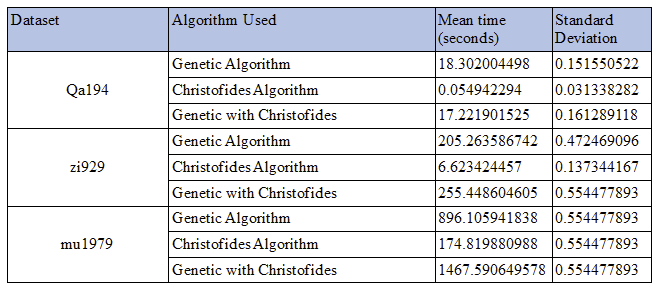
\includegraphics[width=\textwidth]{MeanTime}
	\centering
	\caption{Mean and standard deviations of the time taken by each algorithm over 30 executions}
\end{figure}

Analysing these results is unfortunately not quite as simple as the results before, since they appear to be very peculiar and unflattering. Starting with the qa194 data set we can already spot some strange occurrences, the genetic algorithm completes in around 18 seconds and Christofides algorithm completes in 0.05 seconds. It is expected therefore that the time taken by the hybrid algorithm would be approximately the addition of these times, since that is exactly what the hybrid algorithm is designed to do, it may take longer due to some overhead, yet strangely enough for this smallest data set, the hybrid algorithm takes \textit{less} time to complete than the genetic algorithm, not only this but the standard deviations for the times do not overlap in the slightest. A fair bit of investigation into the code and execution of the program was done in order to try and find the cause of this, yet no reason could be found for this strange occurrence. Given more time further investigation would definitely have to be done to find out the cause of this, as well as the cause of the next few observations.

The second data set shows that the genetic algorithm takes around 205 seconds to complete, Christofides algorithm takes around 6.6 seconds to complete, and yet the hybrid takes 255 seconds. The extra 50 seconds taken are definitely unexpected, and once again the reasoning behind this was truly lost upon investigation of the code.

The same situation was present in the largest data set, yet far worse; the genetic algorithm took 896 seconds, Christofides algorithm 174 seconds and the hybrid a much larger time of 1467 seconds, this implies that the hybrid took around 400 seconds longer than it should have, which is a very extreme increase. 

Not only that, yet the standard deviations for the times in the largest data set and the hybrid in zi929 were all identical. Yet I find this to be far less concerning compared to the mean time in general, since the standard deviations are incredibly low regardless.

All in all, there are some definite unsolved mysteries within these times, and further investigation would be a high priority given more time, as to try and understand where this large overhead is appearing from. If we are to take the results at face value, it is clear to see that the larger datasets take much longer for the hybrid algorithm compared to the algorithms separately. With this in mind it would be important to balance the importance of finding the best result possible with the amount of time taken. mu1979 can achieve a result that is around 7\% off the optimum, compared to Christofides algorithm which would find one that is 10\% worse, for a computation time that is around 10x worse, I certainly admit that it would not be worth this additional time. For the smaller datasets however it may be more useful to wait the additional time, since for the zi929 data set, the hybrid achieved a result that was 6\% better for a time that, whilst still significantly worse than Christofides alone, is still not an incredible length of time. In regards to the smallest data set the hybrid does much better than either alone, and the time is still incredibly small, yet with such a small data set it is uncertain how necessary such a solution is compared to simply using a brute force approach, or the Held-Karp algorithm.

To summarise quite bluntly, I am incredibly dissatisfied with the timings of these algorithms, and think there must be a fundamental flaw lurking somewhere which is causing such a situation, as such finding this and recollecting these results would be my top-most priority in the future, since as it stands the findings within this table are not favourable, and even if they were, such a situation in which there is no clear trend or pattern throws the validity of these timings into question.

\subsection{Multi-Christofides Results}

Unfortunately the results for the multi-Christofides algorithm left much to be desired:

\begin{figure}[ht]
	\begin{subfigure}{.32\textwidth}
		\centering
		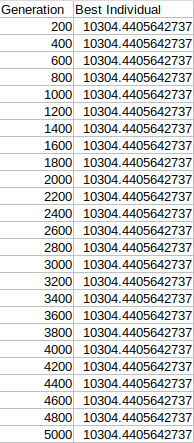
\includegraphics[width=.75\textwidth]{MultQa194}
		\caption{Qa194}
	\end{subfigure}
	\begin{subfigure}{.32\textwidth}
		\centering		
		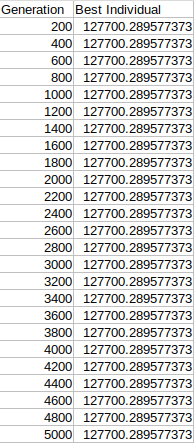
\includegraphics[width=.75\textwidth]{MultZi929}
		\caption{Zi929}
	\end{subfigure}	
	\begin{subfigure}{.32\textwidth}
		\centering
		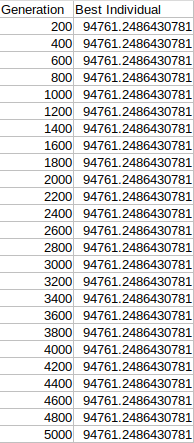
\includegraphics[width=.75\textwidth]{MultMu1979}
		\caption{Mu1979}
	\end{subfigure}
	\centering
	\caption{Evolutionary tables for all three datasets}
\end{figure}

A quick look shows that none of the algorithms had any form of improvement over the 5000 generations, and as such this attempt at bettering our algorithm has failed. The most obvious and likely reason for this is the algorithm previously mentioned that I was not particularly pleased with. It was incredibly difficult to find a way of producing multiple Christofides individuals that were different from one another yet also did not take too long to execute. That function requires a lot more work to be put into it which I was unable to do within this time frame, the function requires some more intelligent implementation of producing individuals that are different from one another, such that we have a much larger spread over the search space. This is because currently it seems all of the produced individuals are very similar, and in fact could be easily produced by the genetic algorithm itself via the mutation and crossover operators. As such, since these individuals are very good in their own right, the genetic algorithm is unable to improve on them, and simply passes all of these individuals to the next generations endlessly, or in other words, we are stuck in a local optima from the second the program began.

As such with additional time it could be beneficial to recreate this algorithm focusing more on producing vastly different individuals, perhaps by checking how many cities are within the same positions in two tours, and picking ones which have as few similarities as possible. However time is a large issue within these algorithms, and so creating said similarity function would take up even more execution time, and a balance needs to be found between running time and the quality of results. Either way the results of this aspect of the project are very disappointing, and working on this given more time would have been preferable, since I still believe this approach to refining the hybrid algorithm has promise.

\section{Conclusion}

I set out on this project in order to investigate the Travelling Salesman Problem, specifically I wished to see how combining existing algorithms would fare in producing results, it was quite clear from the start that the two most obvious algorithms to combine were Christofides algorithm and a genetic algorithm, as no other algorithms seems to have such a logical fit together like these two had. Once this hybrid was produced I wanted to see how it compared to the algorithms it was made of on their own, in both time and quality of results, since for approximation algorithms these two factors are paramount to deciding if an algorithm good or bad.

We can see that in all of the data sets used, the hybrid algorithm was able to produce superior results to the genetic algorithm and Christofides algorithm separately, and this is indeed the preferable result I had hoped for. Not only did it find the best results, but it found those results the most consistently, since the standard deviation for the hybrid algorithm was the lowest across the board, which I didn't expect to be the case at the beginning of this.

The issue and therefore downfall of this project is the time taken, we can see that the hybrid algorithm is (unusually) long, and this is quite a fatal flaw within the project, since the reasoning behind using an approximation algorithm such as this would be to find a good enough result in an appropriate amount of time. The hybrid algorithm ticks the box for 'good enough' yet falls flat on the 'appropriate amount of time' aspect. That being said, as I mentioned within the results analysis I am dissatisfied with the time results, and I believe them to not truly reflect how this algorithm should run, since there is no consistency within the times to claim them as fully valid in my opinion.

What this all means is if you are looking for a good approximate solution to the TSP, this hybrid algorithm is certainly a valid choice, since it is able to get consistently close to the global optimum, as long as time is not a large issue. However if time is an issue then as it stands it would be more beneficial to use Christofides algorithm on its own, yet even this may not be entirely true, since further investigation into the time taken by this algorithm must take place.

It is also interesting to note that this genetic algorithm is a very simple generic one, so a more bespoke or efficient genetic algorithm could fair incredibly well when combined with Christofides algorithm, which is definitely something that could be looked into in the future.

More time would have been very valuable in this project, as mentioned previously there are several things I would have liked to spend more time on, mainly the multiple Christofides function which is considerably flawed, along with further investigation into why the genetic algorithm performed badly on the mu1979 data set and finally a deeper and more accurate investigation into the time taken by the algorithms, as to try and see if the results received now are indeed valid, or if they are entirely incorrect; such an investigation could show that this hybrid algorithm performs much better than what is documented here.

\begin{thebibliography}{1}

\bibitem{TSPWiki}
Wikipedia: Travelling Salesman Problem
\\\url{https://en.wikipedia.org/wiki/Travelling_salesman_problem} (Accessed 20 October 2020)

\bibitem{HeldKarpAlg}
Hutchinson, C. et al. (no date) ‘CMU Traveling Salesman Problem’, p. 25. Available at: \url{https://www.math.cmu.edu/~af1p/Teaching/OR2/Projects/P58/OR2_Paper.pdf} (Accessed: 27 October 2020)

\bibitem{HeldKarpAlg2}
Nguyen, Q. N. (no date) ‘Travelling Salesman Problem and Bellman-Held-Karp Algorithm’, p. 5. Available at: \url{http://www.math.nagoya-u.ac.jp/~richard/teaching/s2020/Quang1.pdf} (Accessed: 12 November 2020)

\bibitem{TSP2020}
Klarreich, E. (no date) Computer Scientists Break Traveling Salesperson Record, Quanta Magazine. Available at: \url{https://www.quantamagazine.org/computer-scientists-break-traveling-salesperson-record-20201008/} (Accessed: 22 October 2020).

\bibitem{ChrAlg}
Christofides, N. (1976) Worst-Case Analysis of a New Heuristic for the Travelling Salesman Problem. CARNEGIE-MELLON UNIV PITTSBURGH PA MANAGEMENT SCIENCES RESEARCH GROUP. Available at: \url{https://apps.dtic.mil/sti/citations/ADA025602} (Accessed: 22 October 2020).

\bibitem{ChrAlgSlides}
Sitters, R. (no date) Chapter 2: Greedy Algorithms and Local Search. Available at: \url{https://personal.vu.nl/r.a.sitters/AdvancedAlgorithms/2016/SlidesChapter2-2016.pdf} (Accessed: 27 October 2020).

\bibitem{ChrAlgSteps}
Christofides algorithm (no date). Available at: \url{https://xlinux.nist.gov/dads/HTML/christofides.html} (Accessed: 27 October 2020).

\bibitem{PvKTime}
Huang, F., Gao, P. and Wang, Y. (2009) ‘Comparison of Prim and Kruskal on Shanghai and Shenzhen 300 Index Hierarchical Structure Tree’, in 2009 International Conference on Web Information Systems and Mining. 2009 International Conference on Web Information Systems and Mining, pp. 237–241. doi: 10.1109/WISM.2009.56.

\bibitem{BlosAlg}
Kolmogorov, V. (2009) ‘Blossom V: a new implementation of a minimum cost perfect matching algorithm’, Mathematical Programming Computation, 1(1), pp. 43–67. doi: 10.1007/s12532-009-0002-8.
Available at: \url{http://mpc.zib.de/archive/2009/1Kolmogorov2009_Article_BlossomVANewImplementationOfAM.pdf} (Accessed: 29 October 2020)

\bibitem{GAIntro}
Melanie, M. (no date) ‘An Introduction to Genetic Algorithms’, p. 162. Available at: \url {http://www.boente.eti.br/fuzzy/ebook-fuzzy-mitchell.pdf} (Accessed: 3 November 2020)

\bibitem{TSPGACrMu}
Penev, M.K.V.S.S., 2005. Genetic operators crossover and mutation in solving the TSP problem. In International Conference on Computer Systems and Technologies. Available at: \url{http://citeseerx.ist.psu.edu/viewdoc/download?doi=10.1.1.83.7264&rep=rep1&type=pdf} (Accessed: 5 November 2020)

\bibitem{GAMutations}
Abdoun, O., Abouchabaka, J. and Tajani, C. (no date) ‘Analyzing the Performance of Mutation Operators to Solve the Travelling Salesman Problem’, p. 18. Available at: \url{https://arxiv.org/pdf/1203.3099.pdf} (Accessed: 5 November 2020)

\bibitem{GACrossover}
Hussain, A. et al. (2017) ‘Genetic Algorithm for Traveling Salesman Problem with Modified Cycle Crossover Operator’, Computational Intelligence and Neuroscience, 2017, pp. 1–7. doi: 10.1155/2017/7430125. Available at: \url{http://downloads.hindawi.com/journals/cin/2017/7430125.pdf} (Accessed: 10 November 2020)

\bibitem{GACrossoverPerformance}
Otman, A. (no date) ‘A Comparative Study of Adaptive Crossover Operators for Genetic Algorithms to Resolve the Traveling Salesman Problem’, International Journal of Computer Applications, 31, p. 9.
Available at: \url{https://arxiv.org/pdf/1203.3097.pdf} (Accessed: 12 November 2020)

\bibitem{TSPRep1}
TSP Test Data (no date). Available at: http://www.math.uwaterloo.ca/tsp/data/index.html (Accessed: 12 November 2020).

\bibitem{TSPRep2}
TSPLIB (no date). Available at: http://comopt.ifi.uni-heidelberg.de/software/TSPLIB95/ (Accessed: 12 November 2020).

\bibitem{DiffAlgs}
Baidoo, E. and O., S. (2016) ‘Solving the TSP using Traditional Computing Approach’, International Journal of Computer Applications, 152(8), pp. 13–19. doi: 10.5120/ijca2016911906. Available at: \url{https://www.researchgate.net/profile/Evans_Baidoo2/publication/309224559_Solving_the_TSP_using_Traditional_Computing_Approach/links/58066b6408ae5ad188166189.pdf} (Accessed: 12 November 2020)

\bibitem{KolMinMatch}
org.jgrapht.alg.matching.blossom.v5 (JGraphT : a free Java graph library) (no date). Available at: https://jgrapht.org/javadoc-1.3.0/org/jgrapht/alg/matching/blossom/v5/package-summary.html (Accessed: 29 April 2021).

\bibitem{HeirEulTour}
HierholzerEulerianCycle (JGraphT : a free Java graph library) (no date). Available at: https://jgrapht.org/javadoc/org.jgrapht.core/org/jgrapht/alg/cycle/HierholzerEulerianCycle.html (Accessed: 29 April 2021).

\end{thebibliography}

\begin{appendices}

\section{Evolutionary Graph Data}
This section shows the full tables of data used to generate the graphs, the only benefit this data gives over the graphs is being able to see the exact values at each generational landmark.
\pagebreak

\subsection{Qa194 Data Table}

\begin{figure}[ht]
	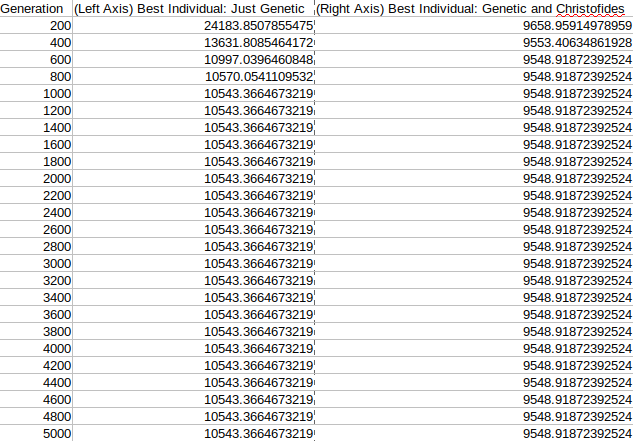
\includegraphics[width=0.75\textwidth]{qa194Table}
	\centering
\end{figure}

\pagebreak

\subsection{Zi929 Data Table}


\begin{figure}[ht]
	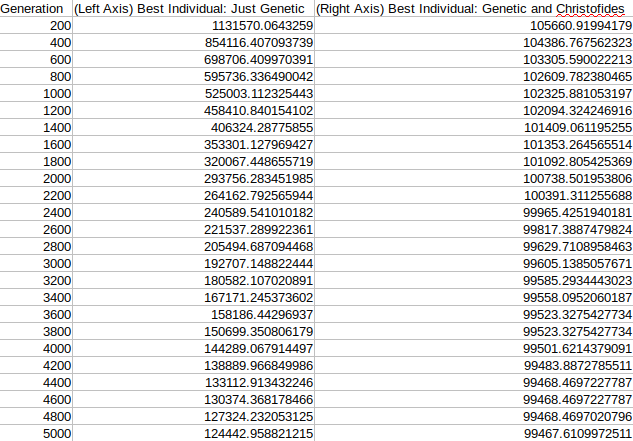
\includegraphics[width=0.75\textwidth]{zi929Table}
	\centering
\end{figure}

\pagebreak

\subsection{Mu1979 Data Table}

\begin{figure}[ht]
	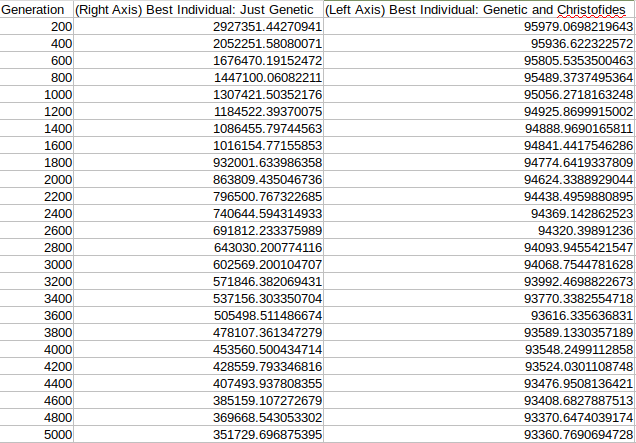
\includegraphics[width=0.75\textwidth]{mu1979Table}
	\centering
\end{figure}
\end{appendices}

\end{document}